\chapter{MARCO TEÓRICO}

\section{Fundamentos y Definición del Problema}

La gestión académica comprende procesos y herramientas para planificar, ejecutar y controlar actividades formativas. En este contexto, la planificación de horarios (\emph{academic timetabling}) es un problema central: asignar clases (asignaturas y grupos) a franjas horarias y espacios cumpliendo restricciones duras (no solapamiento, disponibilidad de aulas y docentes) y optimizando criterios blandos (minimizar tiempos muertos, balancear carga diaria, preferencia de docentes).

Desde la perspectiva de la investigación operativa, el timetabling universitario es típicamente un problema NP–difícil. La complejidad combinatoria crece exponencialmente con el número de materias y grupos, por lo que se emplean estrategias de búsqueda con poda y heurísticas de evaluación multi–criterio \cite{babaei2015-survey,kristiansen2013-survey}.

En la Facultad de Ciencias y Tecnología de la UMSS, los horarios se publican semestralmente en formato PDF en el portal institucional \cite{horarios_fcyt}. Este formato limita la personalización, complica la consulta móvil y no provee alertas ni verificación automática de conflictos. Estas limitaciones motivan soluciones móviles especializadas que soporten organización dinámica, validación de conflictos y funcionamiento offline.

\section{Formalización Matemática del Problema para un Usuario}

El caso de TecnoTime está centrado en un único estudiante: se selecciona el mejor conjunto de grupos para sus materias, sin modelar múltiples estudiantes ni capacidades institucionales. Por ello se usa un modelo de \emph{selección de grupos} más simple que el institucional.

\subsection*{Modelo de Selección de Grupos}
\begin{itemize}
  \item Conjuntos: materias del usuario \(C\). Para cada materia \(c\), su conjunto de grupos ofertados \(G(c)\). Días \(W\) y franjas temporales \(T\) (para definir solapes).
  \item Variable de decisión binaria: \(y_{c,g}=1\) si el usuario elige el grupo \(g\in G(c)\) para la materia \(c\); en otro caso, \(0\).
  \item Horarios preexistentes: cada par \((c,g)\) tiene un conjunto de intervalos temporales \(\text{sched}(c,g)\) (día, inicio, fin) obtenido del PDF.
\end{itemize}

Restricciones duras (usuario):
\begin{align}
  &\text{Una opción por materia: } \forall c\in C:\ \sum_{g\in G(c)} y_{c,g} \;=\; 1 \\[-2pt]
  &\text{Sin solapes: } \forall (c_1,g_1)\neq(c_2,g_2):\ \big(\text{overlap}(\text{sched}(c_1,g_1),\,\text{sched}(c_2,g_2))\big) \Rightarrow y_{c_1,g_1}+y_{c_2,g_2}\;\le\;1
\end{align}

Restricciones blandas (preferencias del usuario): minimizar huecos intra–día, ajustar n.º de días activos y priorizar docentes favoritos.

Función objetivo multi–criterio (suma ponderada) \cite{deb2001-moo,charnes1961-gp}:
\begin{equation}
  \min_{y}\ F(y)= \sum_{k} w_k\, \phi_k(y),\quad w_k\ge 0
\end{equation}

\subsection*{Tabla de Notación} \label{tab:notacion-uctp}
\begin{table}[H]
  \centering
  \small
\begin{tabular}{>{\bfseries}m{2.6cm} m{7.4cm} m{3cm}}
    \hline
    Símbolo & Significado & Dominio \\
    \hline
    $C,G,D,R,T,W$ & Conjuntos de materias, grupos, docentes, aulas, franjas, días & Finito \\
    $y_{c,g}$ & Selección de grupo para materia $c$ & $\{0,1\}$ \\
    $\text{sched}(c,g)$ & Conjunto de intervalos (d\'\i a, inicio, fin) & $\mathcal{I}$ \\
    $\text{overlap}(\cdot,\cdot)$ & Predicado de solape temporal & $\{\text{true,false}\}$ \\
    $\text{doc}(c,g)$ & Docente del grupo $g$ de $c$ & $-$ \\
    $\text{calendar}(t)$ & Slot a (d\'\i a, inicio, fin) & $W\times \mathbb{T}$ \\
    $\phi_k(y)$ & Penalización del criterio $k$ & $\mathbb{R}_{\ge 0}$ \\
    $w_k$ & Peso del criterio $k$ & $\mathbb{R}_{\ge 0}$ \\
    \hline
  \end{tabular}
  \caption{Notación básica para la formalización del UCTP. Completar según el caso de estudio.}
\end{table}

\subsection*{Tabla de Restricciones (enfoque usuario)}
\begin{table}[H]
  \centering
  \small
  \begin{tabular}{>{\bfseries}m{2.0cm} m{7.1cm} m{4.3cm} m{2.0cm}}
    \hline
    Tipo & Descripción & Formalización (borrador) & Fuente de dato \\
    \hline
    Dura & Una opción por materia & $\forall c:\ \sum_{g\in G(c)} y_{c,g}=1$ & Materias del usuario \\
    Dura & No solape entre grupos & $y_{c_1,g_1}+y_{c_2,g_2}\le 1$ si $overlap$ & Horarios ofertados \\
    Blanda & Minimizar gaps & $\sum\text{minutos\_vac\'\i os}(y)$ & Preferencias \\
    Blanda & Ajustar d\'\i as activos & $\sum\mathbf{1}[\text{d\'\i a con clases}]$ & Preferencias \\
    Blanda & Docentes favoritos & $\sum \mathbf{1}[\neg favorito]$ & Preferencias \\
    \hline
  \end{tabular}
  \caption{Clasificación de restricciones duras y blandas. Adaptar a la instancia real.}
\end{table}

\section{Representación de Datos Académicos}

Un modelo de datos consistente es condición para expresar restricciones y evaluar soluciones. A nivel conceptual (E/R) se consideran las siguientes entidades y asociaciones: Carrera, Nivel, Asignatura, Grupo, Horario de Grupo, Docente, Aula, Selección del Estudiante y Eventos Académicos. Las relaciones N:M entre Carrera–Nivel, Carrera–Grupo y Asignatura–Grupo se resuelven con tablas de cruce para evitar redundancia y habilitar consultas eficientes \cite{chen1976-er,codd1971-3nf}.

Principios teóricos aplicados:
\begin{itemize}
  \item Normalización hasta 3FN para evitar anomalías de inserción, actualización y eliminación.
  \item Integridad referencial mediante claves foráneas con políticas \emph{CASCADE} o \emph{SET NULL} según opcionalidad.
  \item Índices compuestos en claves de búsqueda frecuentes (p.ej. \texttt{(subject\_code, group\_id)}), como soporte para restricciones y validaciones.
\end{itemize}

A nivel lógico, los ORMs modernos (p.ej., Room) proveen DAOs tipadas y validación de esquemas en tiempo de compilación \cite{room_db}. Estas herramientas no constituyen metodología de desarrollo en este capítulo, sino sustento tecnológico del modelo de datos que hace posible la expresión de restricciones y la evaluación de soluciones.

\subsection*{Diagrama ER}
\begin{figure}[H]
  \centering
  \includegraphics[width=\linewidth]{images/diagram_er.png}
  \caption{Diagrama ER del dominio académico. Fuente: \cite{tecnotime-er-dbdiagram}.}
  \label{fig:er}
\end{figure}

\subsection*{Tabla de Entidades e Índices (resumen)}
\begin{table}[H]
  \centering
  \small
  \begin{tabular}{>{\bfseries}m{2.6cm} m{5.5cm} m{4.7cm}}
    \hline
    Entidad & Claves (PK/FK) & Índices / Notas \\
    \hline
    Materia & PK: code & UNIQUE(code), b\'usqueda por nombre \\
    Grupo & PK: id, FK: subject\_code, level\_id & UNIQUE(subject\_code, group\_id) \\
    HorarioGrupo & PK: id, FK: group\_id, teacher\_id, classroom\_id & (teacher\_id, day, start), (classroom\_id, day, start) \\
    Docente & PK: id & UNIQUE(full\_name) \\
    Aula & PK: id & UNIQUE(name) \\
    Selección & PK: id, FK: subject/group & Preferencias, color, emoji \\
    \hline
  \end{tabular}
  \caption{Resumen de entidades, claves e índices (completar/ajustar).}
\end{table}

\section{Fundamentos Algorítmicos para la Generación de Horarios}

La generación de horarios puede formalizarse como un problema de búsqueda combinatoria con evaluación multi–objetivo. Dos componentes teóricos son fundamentales: el mecanismo de exploración de combinaciones y la función de evaluación.

\subsection{Exploración: Búsqueda con Retroceso (Backtracking)}

El backtracking explora sistemáticamente combinaciones de grupos por materia. La poda temprana descarta ramas que violan restricciones duras (solapamientos, disponibilidad de docente/aula). Esta técnica garantiza cobertura del espacio factible a costa de complejidad exponencial en el peor caso; la poda y el ordenamiento heurístico de variables y valores reducen el espacio efectivo \cite{golomb1965-backtrack}.

\subsection*{Pseudocódigo de Backtracking (borrador)}
\begin{lstlisting}[language={},basicstyle=\ttfamily\small]
func generarHorarios(candidatos, estrategia, N):
    mejores = []
    def backtrack(i, parcial):
        if i == len(candidatos):
            score = estrategia(parcial)
            insertar_ordenado(mejores, (parcial, score), N)
            return
        for opcion in candidatos[i]:
            if cumple_duras(parcial + opcion):   # poda temprana
                backtrack(i+1, parcial + opcion)
    backtrack(0, [])
    return extraer_horarios(mejores)
\end{lstlisting}

\subsection*{Diagrama de flujo del algoritmo (TikZ)}
\begin{figure}[H]
  \centering
  \resizebox{\linewidth}{!}{%
  \begin{tikzpicture}[
    node distance=10mm,
    every node/.style={font=\small},
    box/.style={rectangle, draw, rounded corners, align=center, minimum width=38mm, minimum height=7mm},
    decision/.style={diamond, draw, aspect=2, align=center, inner sep=1pt}
  ]
    \shorthandoff{< >}% desactiva guillemets de babel en este entorno
    \node[box] (start) {Ordenar materias (MRV)};
    \node[box, below=of start] (pick) {Seleccionar materia i};
    \node[box, below=of pick] (iter) {Iterar grupos (LCV)};
    \node[decision, below=of iter] (hard) {Cumple\newline duras?};
    \node[box, below left=13mm and 18mm of hard] (prune) {Poda y retroceso};
    \node[box, below right=13mm and 18mm of hard] (add) {Agregar a parcial};
    \node[decision, below=20mm of add] (done) {i = |C|?};
    \node[box, below right=13mm and 18mm of done] (eval) {Evaluar y mantener\newline Top-N};
    \node[box, below left=13mm and 18mm of done] (advance) {i \(\leftarrow\) i+1};

    \draw (start) -- (pick);
    \draw (pick) -- (iter);
    \draw (iter) -- (hard);
    \draw (hard.west) -- ++(-10mm,0) |- (prune);
    \draw (hard.east) -- ++(10mm,0) |- (add);
    \draw (add) -- (done);
    \draw (done.east) -- ++(10mm,0) |- (eval);
    \draw (done.west) -- ++(-10mm,0) |- (advance);
    \draw (advance) |- (iter);
  \end{tikzpicture}}
  \caption{Flujo de backtracking con MRV/LCV, poda de duras y mantenimiento de Top-N.}
\end{figure}

\subsection{Evaluación: Heurísticas y Multi–criterio}

El sistema de evaluación asigna una puntuación a un horario completo según múltiples objetivos blandos. Criterios típicos, coherentes con las necesidades del dominio, incluyen:
\begin{itemize}
  \item Minimizar huecos entre clases por día (\emph{gaps}).
  \item Minimizar días sin clases cuando el usuario prefiere concentración.
  \item Penalizar conflictos si no están permitidos; tolerarlos si el usuario lo acepta de forma explícita.
  \item Priorizar docentes marcados como favoritos.
\end{itemize}

Una forma general es una combinación lineal ponderada de estrategias específicas (\emph{Composite Strategy}), lo que habilita ajuste de preferencias del usuario sin redefinir el algoritmo de búsqueda \cite{deb2001-moo,charnes1961-gp}.

\subsection*{Tabla de Métricas y Pesos}
\begin{table}[H]
  \centering
  \small
  \resizebox{\linewidth}{!}{%%
  \begin{tabular}{>{\bfseries}m{2.6cm} m{5.0cm} m{2.1cm} m{2.8cm} m{1.6cm}}
    \hline
    Métrica & Fórmula (bosquejo) & Rango & Interpretación & Peso $w_k$ \\
    \hline
    Conflictos & $\infty$ si hay solapamientos, $0$ si no & $\{0,\infty\}$ & Cr\'\i tico (prohibido) & 1.0 \\
    Gaps (min) & $\sum\limits_{d\in W}\sum\limits_{i} \max(0, s_{i+1}-e_i)$ & $[0,600]$ & Menor es mejor & 1.0 \\
    Docentes no fav. & $\sum \mathbf{1}[\neg favorito]$ & $[0,n]$ & Penaliza no favoritos & 1.0 \\
    D\'\i as vac\'\i os & $\sum\limits_{d\in W} \mathbf{1}[|clases(d)|=0]$ & $[0,6]$ & Preferible menos & 0.5 \\
    \hline
  \end{tabular}%%
  }
  \caption{Métricas de evaluación y pesos (ajustar y normalizar según preferencia).}
\end{table}

\noindent Función objetivo global de ejemplo:
\begin{equation}
  F(H)=1.0\cdot\text{conflicts}(H)+1.0\cdot\text{gaps}(H)+1.0\cdot\text{teachers}(H)+0.5\cdot\text{days}(H)
\end{equation}

\section{Complejidad y Relación Teórica}

El UCTP es \emph{NP–dif\'\i cil} \cite{babaei2015-survey,kristiansen2013-survey}. La exploración por backtracking tiene complejidad \(O(b^d)\), donde \(b\) es el factor de ramificación (grupos por materia) y \(d\) la profundidad (número de materias). La poda y heur\'\i sticas como MRV y LCV reducen el espacio efectivo \cite{golomb1965-backtrack}. El problema se relaciona con coloreo de grafos (clases como nodos, slots como colores) y scheduling por intervalos.

\subsection*{L\'inea de tiempo (TikZ) y c\'alculo de gaps}
\begin{figure}[H]
  \centering
  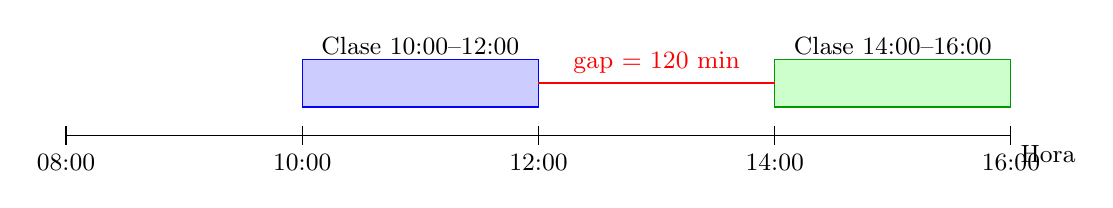
\begin{tikzpicture}[x=3mm,y=6mm, every node/.style={font=\small}]
    \shorthandoff{< >}% desactiva guillemets de babel en este entorno
    % Eje de tiempo 08:00 a 16:00 (ajustado a ancho)
    \draw (0,0) -- (40,0) node[below right]{Hora};
    \foreach \x/\h in {0/08:00,10/10:00,20/12:00,30/14:00,40/16:00}
      \draw (\x,0.2) -- (\x,-0.2) node[below]{\h};
    % Bloques de clase de la mini-instancia (Martes 10-12 y 14-16)
    \filldraw[fill=blue!20,draw=blue] (10,0.6) rectangle (20,1.6);
    \node at (15,1.9) {Clase 10:00–12:00};
    \filldraw[fill=green!20,draw=green!60!black] (30,0.6) rectangle (40,1.6);
    % ticks principales hasta 16:00 ya agregados
    \node at (35,1.9) {Clase 14:00–16:00};
    % Gap indicado
    \draw[red,thick] (20,1.1) -- (30,1.1);
    \node[above,red] at (25,1.1) {gap = 120 min};
  \end{tikzpicture}
  \caption{Ejemplo de c\'alculo de gaps intra–d\'ia (Martes: 10–12 y 14–16).}
\end{figure}

\section{Patrones y Principios de Arquitectura de Software}

Las decisiones de arquitectura se fundamentan en teoría de diseño de software, con impacto directo sobre mantenibilidad, escalabilidad y testabilidad, sin entrar en metodologías de proceso.

\subsection{Clean Architecture y MVVM}

Clean Architecture separa responsabilidades en capas concéntricas (Presentación, Dominio, Datos), de modo que los detalles dependen de abstracciones. MVVM aporta un patrón de separación de la lógica de presentación de la UI. Estos enfoques reducen acoplamiento, facilitan pruebas y permiten evolucionar componentes sin afectar la lógica de negocio \cite{pedreira2021comparativa, medina2014, martin2017-cleanarch}.

\subsection{Repository, DAO y Principio de Inversión de Dependencias}

El patrón Repository abstrae el acceso a datos; los DAOs tipados proveen operaciones declarativas. El Principio de Inversión de Dependencias (DIP) garantiza que la capa de dominio no dependa de detalles de infraestructura. Este andamiaje teórico permite sustituir fuentes de datos (locales o remotas) sin impacto en la lógica central.

\subsection{Patrón Strategy para Evaluación de Horarios}

El patrón Strategy encapsula criterios de evaluación (\emph{minimizar gaps}, \emph{priorizar docentes}, etc.) bajo una interfaz común, habilitando su composición y extensión sin modificar el generador de combinaciones. Esta separación favorece pruebas unitarias de cada criterio y mezcla de preferencias del usuario \cite{gamma1995-patterns,fowler2002-peaa}.

\subsection{Notificaciones y Trabajo Diferido}

Las notificaciones locales y el trabajo diferido en segundo plano son conceptos de plataforma que respaldan recordatorios oportunos de clases y eventos. Su inclusión en el marco teórico se justifica por su función como mecanismo de entrega de información contextual y por los modelos de ejecución diferida de sistemas operativos móviles.

\section{Obtención de Datos: Web Scraping y Parsing de PDF}

Como fuente oficial de información, la FCyT publica horarios en PDF \cite{horarios_fcyt}. Para llevar estos datos a un modelo estructurado, se recurre a técnicas de web scraping y parsing:
\begin{itemize}
  \item Extracción de enlaces y metadatos desde páginas HTML institucionales.
  \item Descarga de PDFs y lectura de contenido para extraer asignaturas, grupos, docentes, aulas y franjas horarias.
  \item Limpieza, validación y normalización de datos para persistencia local y consulta eficiente.
\end{itemize}

Aspectos teóricos relevantes incluyen: límites éticos y legales del scraping institucional, manejo de cambios en el origen (robustez a variaciones de formato), y trazabilidad de la fuente \cite{mitchell2018-scraping,smith2007-tesseract}.

\subsection*{Pipeline de datos (TikZ)}
\begin{figure}[H]
  \centering
  \resizebox{\linewidth}{!}{%
  \begin{tikzpicture}[
    node distance=10mm,
    every node/.style={font=\small},
    stage/.style={rectangle, draw, align=center, minimum width=36mm, minimum height=7mm}
  ]
    \shorthandoff{< >}% desactiva guillemets de babel en este entorno
    \node[stage] (nweb) {Web\newline (HTML/PDF)};
    \node[stage, right=20mm of nweb] (nparse) {Extracci\'on\newline (scraping/parsing)};
    \node[stage, right=20mm of nparse] (nclean) {Limpieza\newline y normalizaci\'on};
    \node[stage, below=12mm of nclean] (ner) {Modelo ER};
    \node[stage, left=20mm of ner] (ngen) {Generaci\'on\newline (backtracking)};
    \node[stage, left=20mm of ngen] (neval) {Evaluaci\'on\newline (m\'etricas y pesos)};
    \node[stage, below=12mm of ngen] (nres) {Horarios\newline candidatos};

    \draw (nweb) -- (nparse);
    \draw (nparse) -- (nclean);
    \draw (nclean) -- (ner);
    \draw (ner) -- (ngen);
    \draw (ngen) -- (neval);
    \draw (ngen) -- (nres);
    \draw (neval) -- (nres);
  \end{tikzpicture}}
  \caption{Flujo de datos: desde la fuente institucional hasta horarios evaluados.}
\end{figure}

\section*{Mini-instancia de ejemplo (para figuras/tablas)}
\noindent\textbf{Dataset de ejemplo:} 3 materias con 2 grupos cada una.
\begin{table}[H]
  \centering
  \small
  \begin{tabular}{l l l l l l l r}
    \hline
    Materia & Grupo & Docente & D\'\i a & Inicio & Fin & Aula & Cap. \\
    \hline
    MAT1 & G1 & P\'erez  & Lunes     & 08:00 & 10:00 & A101 & 30 \\
    MAT1 & G2 & L\'opez  & Martes    & 10:00 & 12:00 & A102 & 25 \\
    MAT2 & G1 & P\'erez  & Lunes     & 10:00 & 12:00 & A101 & 30 \\
    MAT2 & G2 & Garc\'\i a & Mi\'ercoles & 08:00 & 10:00 & A103 & 40 \\
    MAT3 & G1 & L\'opez  & Martes    & 14:00 & 16:00 & A102 & 25 \\
    MAT3 & G2 & Garc\'\i a & Jueves    & 10:00 & 12:00 & A103 & 40 \\
    \hline
  \end{tabular}
  \caption{Mini-conjunto para ilustrar conflictos y c\'alculo de m\'etricas.}
\end{table}

\noindent\textbf{C\'alculo de m\'etricas (ejemplo):}
\begin{itemize}
  \item Horario A: (MAT1-G1, MAT2-G1, MAT3-G1). Gaps: 120 min (Martes). D\'\i as activos: 2. Docentes no fav.: 1 (L\'opez). Score: $0 + 120 + 1 + 0.5\cdot(6-2) = 123$.
  \item Horario B: (MAT1-G2, MAT2-G2, MAT3-G2). Gaps: 120 min. D\'\i as activos: 3. Docentes no fav.: 2. Score: $0 + 120 + 2 + 0.5\cdot(6-3) = 123.5$.
\end{itemize}

\section{Estado del Arte y Referentes}

En el ámbito local, el sistema Cappuccino (S.C.E.S.I.) ofrece organización de horarios vía web, con alcance institucional pero sin personalización móvil avanzada \cite{cappuccino_umss}. En el ámbito internacional/comercial, aplicaciones como Smart Timetable incorporan generación de horarios, recordatorios y sincronización en la nube \cite{smart_timetable}. Asimismo, existen soluciones institucionales de timetabling de mayor escala, como UniTime y FET, que atienden el problema a nivel institucional con restricciones y alcances distintos al enfoque personal \cite{unitime-ref,fet-ref}.

Este estado del arte evidencia la pertinencia de combinar: optimización de horarios centrada en el usuario, soporte offline, notificaciones y exportación/compartición de resultados, dentro de una arquitectura mantenible.

\section{Síntesis}

El marco teórico de TecnoTime se apoya en: (i) la formalización del timetabling académico como problema NP–difícil y la aplicación de búsqueda con poda más evaluación multi–criterio; (ii) un modelo de datos normalizado que expresa entidades y restricciones del dominio; (iii) patrones de arquitectura (Clean Architecture, MVVM, Repository, Strategy) que reducen acoplamiento y habilitan extensibilidad; y (iv) técnicas de scraping/parsing que conectan la fuente institucional de datos con el modelo estructurado. Estas bases conceptuales justifican y guían las decisiones técnicas del proyecto, sin constituir metodología de desarrollo, y dejan abiertos frentes de investigación bibliográfica específicos para consolidar citas canónicas donde se marcó “investigar y completar”.
